\chapter{Descriptions techniques}

\section{Dépendances et librairies externes utilisées}

Afin de pouvoir implémenter une partie de nos fonctionnalités principales et d'optimiser l'expérience utilisateur de l'application, nous avons eu à faire recours à plusieurs bibliothèques externes. Pour cela, il a avant tout fallu se documenter à propos des bibliothèques existantes et avoir des avis sur celles-ci afin de s'assurer qu'elles soient bien stables, à jour, et qu'elles fournissent tous les services qui nous sont nécessaires.\\

L'application utilise cinq bibliothèques externes: \\

\begin{itemize}
\renewcommand{\labelitemi}{$\bullet$}
\item \textbf{UnboundID LDAP SDK}~\cite{unboundId}: indispensable pour la connexion aux serveurs utilisant le protocole LDAP étant donné que la SDK de Java ne fournit aucun outil équivalent. On avait également encore le choix avec \textit{JNDI LDAP} et \textit{Spring LDAP} qui sont deux bibliothèques connues mais obsolètes et beaucoup plus complexes à utiliser. \\
\item \textbf{Jsoup}~\cite{jsoup}: la bibliothèque de référence pour l'analyse textuelle de textes HTML et XML. Elle est utilisée pour parser les événements des deux établissements ainsi que l'annuaire du LaBRI. \\
\item \textbf{Google Play Services}: bibliothèque nécessaire pour utiliser les services de Google Maps et donc implémenter les services affectant le plan du campus. \\
\item \textbf{Sliding Menu}~\cite{slidingMenu}: bibliothèque open-source qui sert à améliorer l'esthétique et l'expérience utilisateur au sein du service qui affiche les événements. Elle permet de rajouter un menu latéral qui sert à basculer entre les différentes catégories d'événements à tout moment en faisant un simple geste de glissement avec le doigt. \\
\item \textbf{Robotium}~\cite{robotium}: bibliothèque open-source spécifique à la plateforme Android qui nous a été utile durant la phase finale du projet afin d'effectuer des tests en boîte noire pour notre interface graphique. 
\end{itemize}

\section{Recyclage de vues dans ListView}
Android fournit des outils pour la gestion des listes graphiques, notamment ListView couplée avec l’interface ListAdapter.\\
ListView est conçue pour être extensible et performante, ce qui signifie:

\begin{enumerate}
\item ListView va essayer d’effectuer des inflations de vues aussi peu que possible.
\item ListView ne va dessiner et disposer ses fils que quand ils sont visibles sur l’écran (ou sur le point de l'être).
\end{enumerate}

\wl Le point 1 se justifie par le fait que les opérations d’inflation de layout sont coûteuses (de l’ordre de 1kB de RAM par vue). Ce problème est résolu par le recyclage des vues non visibles, qu’on appelle \emph{ScrapView}. Cela signifie qu’on peut utiliser des vues recyclées et les mettre à jour, au lieu de faire des inflations de vues pour chaque rangée.

Afin d’implémenter le point 2, ListView utilise un recycleur de vues qui déplacera les vues actives dans une pool recyclable quand elles sortent de l’écran. 
Ainsi, ListView n'a besoin de garder en mémoire que les vues visibles à l'écran, ainsi que quelques vues recyclées - même quand ListAdapter contient des centaines d'items. \\

\begin{figure}[h!]
  \center
  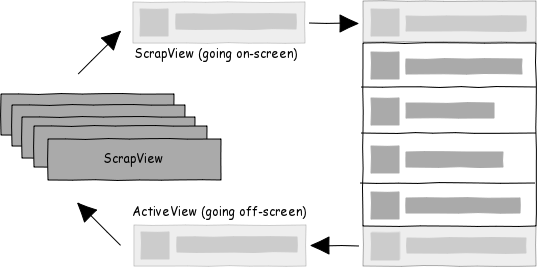
\includegraphics[width=0.55\textwidth]{resources/listview_recycling.png}
  \caption{Recyclage de vues lors du déroulement de ListView vers le bas}
  \label{fig:listview_recycling}
\end{figure}

\newpage
\subsection*{Implémentation de getView()}

A chaque fois que ListView a besoin d’afficher une nouvelle ligne sur l’écran, elle appelle la méthode \emph{getView()} depuis son adapter.

\begin{adjustbox}{minipage=1.14\textwidth,margin=0pt \smallskipamount,center}
\begin{lstlisting}[style=Java, label=listview1, caption=Version naïve]
public View getView(int position, View convertView, ViewGroup parent){ 
	View item = mInflater.inflate(R.layout.item, null);
	((TextView) item.findViewById(R.id.text)).setText(DATA[position]); 
	((ImageView) item.findViewById(R.id.icon)).setImageBitmap(mIcon);
	return item; 
}
\end{lstlisting}
\end{adjustbox}

\wl L’argument \emph{convertView} est essentiellement une vue recyclée (\emph{ScrapView}), comme indiqué précédemment. Quand il a une valeur non nulle, il faut en profiter pour simplement mettre à jour les données au lieu de faire une nouvelle inflation de layout. On peut donc optimiser le processus en employant ce paramètre:

\begin{adjustbox}{minipage=1.14\textwidth,margin=0pt \smallskipamount,center}
\begin{lstlisting}[style=Java, label=listview2, caption=Version correcte]
public View getView(int position, View convertView, ViewGroup parent){ 
	View item = converView;
	if (item != null) {
		item = mInflater.inflate(R.layout.item, parent, false);
	}
	((TextView) item.findViewById(R.id.text)).setText(DATA[position]); 
	((ImageView) item.findViewById(R.id.icon)).setImageBitmap(mIcon);
	return item; 
}
\end{lstlisting}
\end{adjustbox}

\newpage
\subsection*{View Holder pattern}
L'opération de recherche d'une vue dans un layout s'effectue à l'aide de la méthode \emph{findViewById()}. Cette méthode va chercher récursivement dans l'arbre des vues le nœud correspondant à l'ID spécifié. Comme ListView appelle souvent la méthode \emph{getView()} de son adapter lorsqu'on défile la liste, \emph{findViewById()} peut devenir alors assez coûteuse.\\
Le pattern View Holder consiste alors à réduire les appels de \emph{findViewById()} dans \emph{getView()}. Il s'agit donc d'une classe interne légère qui maintient des références directes à toutes les vues internes d'une rangée de la liste, et qu'on peut la stocker en tant que \emph{tag} dans la vue de la rangée.\\

\begin{adjustbox}{minipage=1.14\textwidth,margin=0pt \smallskipamount,center}
\begin{lstlisting}[style=Java, label=listview3, caption=Version optimisée]
static class ViewHolder {
	TextView text;
	ImageView icon;
}

public View getView(int position, View convertView, ViewGroup parent){ 
	ViewHolder holder;

	if (convertView != null) {
		convertView = mInflater.inflate(R.layout.item, parent, false);
		holder = new ViewHolder();
		holder.text = (TextView) convertView.findViewById(R.id.text);
		holder.icon = (ImageView) convertView.findViewById(R.id.icon);
		convertView.setTag(holder)
	} else {
		holder = (ViewHolder) convertView.getTag();
	}
	holder.text.setText(DATA[position]); 
	holder.icon.setImageBitmap(mIcon);
	return convertView; 
}
\end{lstlisting}
\end{adjustbox}

\newpage
En mesurant les performances des 3 implémentations précédentes, on arrive à 20 FPS pour la version naïve, 50 FPS pour la version correcte, et 55 FPS pour la version optimisée.\\

\begin{figure}[h]
  \center
  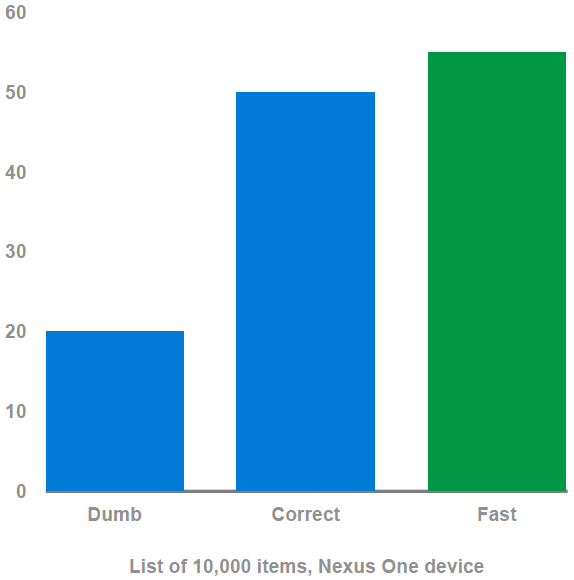
\includegraphics[width=0.6\textwidth]{resources/google_io_2010.png}
  \caption{Performance de \emph{getView()} en fonction des implémentations. Source: Google I/O 2010 - The world of ListView.}
  \label{fig:google_io_2010}
\end{figure}
